\chapter{Metodologia}
\addcontentsline{toc}{chapter}{Metodologia}

\section{Classificação da Pesquisa}

Neste capitulo iremos definir a metodologia estabelecida\ 
para essa pesquisa, bem como a fonte dos dados utilizados,\ 
os trabalhos relacionados, de onde buscamos o referêncial teórico,\
além da classificação da pesquisa em si.

Esta pesquisa pode ser classificada, do ponto de vista de sua natureza,\ 
como aplicada, uma vez que a apartir dos conhecimentos bibliográficos,\
iremos propor um modelo probabilistico para inferência de fraquezas\
de software, a partir de variáveis como a linguagem do projeto e o \
seu tamanho(medido por sloccount). Do ponto de vista da forma de abordagem,\
podemos classificá-la como quantitativa, pois a inferência realizada\ 
utilizando os pacotes debian será feita por técnicas estatísticas.

Alinhada aos objetivos do trabalho, esta pesquisa é exploratória, \ 
e se constroi a apartir dos estudos realizados na área de \ 
aprendizado de máquina.

Do ponto de vista dos procedimentos técnicos, \ 
esta pesquisa é bibliográfica e experimental.

\section{Trabalhos relacionados}

A área de aprendizado de máquina é bastante vasta, e aplicável a \ 
diferentes domínios.
Durante o levantamento bibliográfico encontrou-se diversos \ 
sistemas que fazem uso de aprendizado de máquina e que possuem certa \ 
similaridade com o que será proposto por essa pesquisa.\
Um primeiro trabalho relacionado que podemos citar, é a utilização de \ 
técnicas de aprendizado de máquina para classificar modulos e classes \ 
como passíveis, ou não, a falha\cite{Malhotra}.
A construção de um modelo que represente esse tipo de contexto, \ leva em \ 
consideração métricas de código fonte e dados previos de falhas\cite{Malhotra}.

Para o domínio de pacotes debian aliado ao uso de um modelo grafico \ 
probabilístico que tenha como fonte de dados estes pacotes, \ 
podemos citar a Aplicação \textit{AppRecommender}. Essa aplicação recomenda \ 
pacotes Debian para o usuário, a partir da criação de um perfil, \ 
estabelecido utilizando os pacotes manualmente instalados na máquina.
O processo de recomendação faz uso do algorítmo de bayes, e a fase de \ 
treinamento do algorítmo foi feita coletando dados de vários \ 
usuários da distribuição Debian.

%TODO: Dar exemplo de projetos que utilizam inferência

\section{Coleta de dados}
Os dados que serão utilizados nessa pesquisa, serão em \ 
parte dados primários e em parte dados secundários. Os dados secundários \ 
serão utilizados na fase de treinamento do aprendizado de máquina, \ 
buscando encontrar o melhor modelo estatístico que traduza o \ 
domínio com que estamos lidando. Os dados primários serão \ 
coletados a partir da implantação de algumas ferramentas, que \ 
farão parte da construção dessa pesquisa.

\subsection{Sate}
Os dados secundários foram obtidos por meio do projeto $Sate$. \ 
Nesse projeto, várias ferramentas de análise estática foram executadas \ 
em diferentes projetos. O resultado obtido por essas ferramentas foi \ 
agrupado em uma linguagem única, e disponiblizado em \ 
formato $xml$ na internet. Essa padronização foi feita pelo fato \ 
de que cada ferramenta utilizada na fase de coleta, gerava uma \ 
saída diferente, dificultando a análise feita pelos pesquisadores. \ 
O projeto $Sate$ durou de 2008 até 2012, sendo que a cada ano de projeto, \ 
um conjunto de dados análisados e um relatório da pesquisa foram \ 
disponibilizados(O ano de 2011 não possui dados e também não possui relatório).

\newpage
\begin{figure}[h]
	\centering
	\label{sate_schema}
        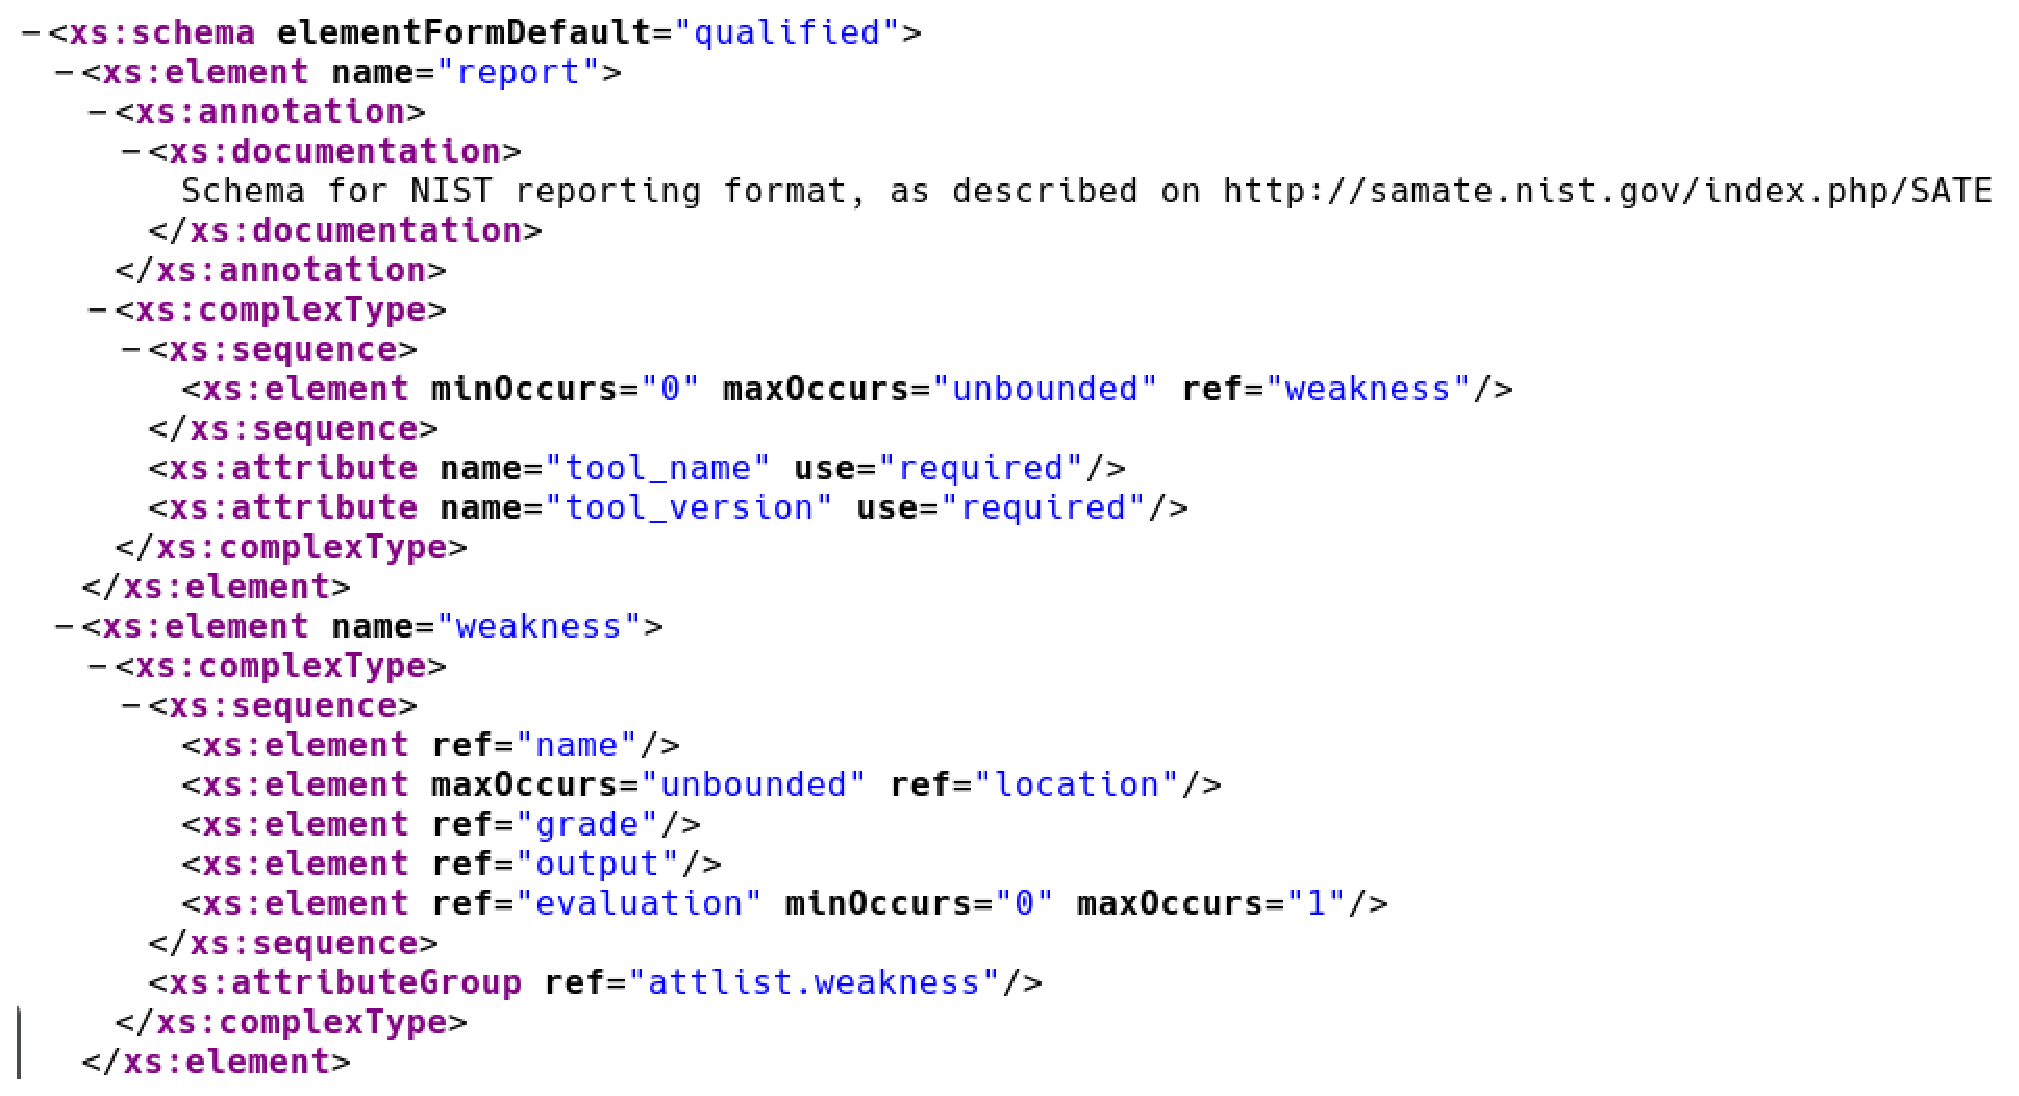
\includegraphics[scale=0.42]{figuras/sate_schema.eps}
	\caption{O padrão xml que as ferramentas que \
        participaram do projeto adotaram}
\end{figure}

A partir do uso do esquema definido na figura~\ref{sate_schema}, \ 
foi possível definir um processo de análise do relatório \
gerado pelas diferentes ferramentas escolhidas. Um exemplo de \ 
relatório padronizado da ferramenta $cppcheck$, utilizada no projeto.

\begin{figure}[h]
	\centering
	\label{cppcheck}
        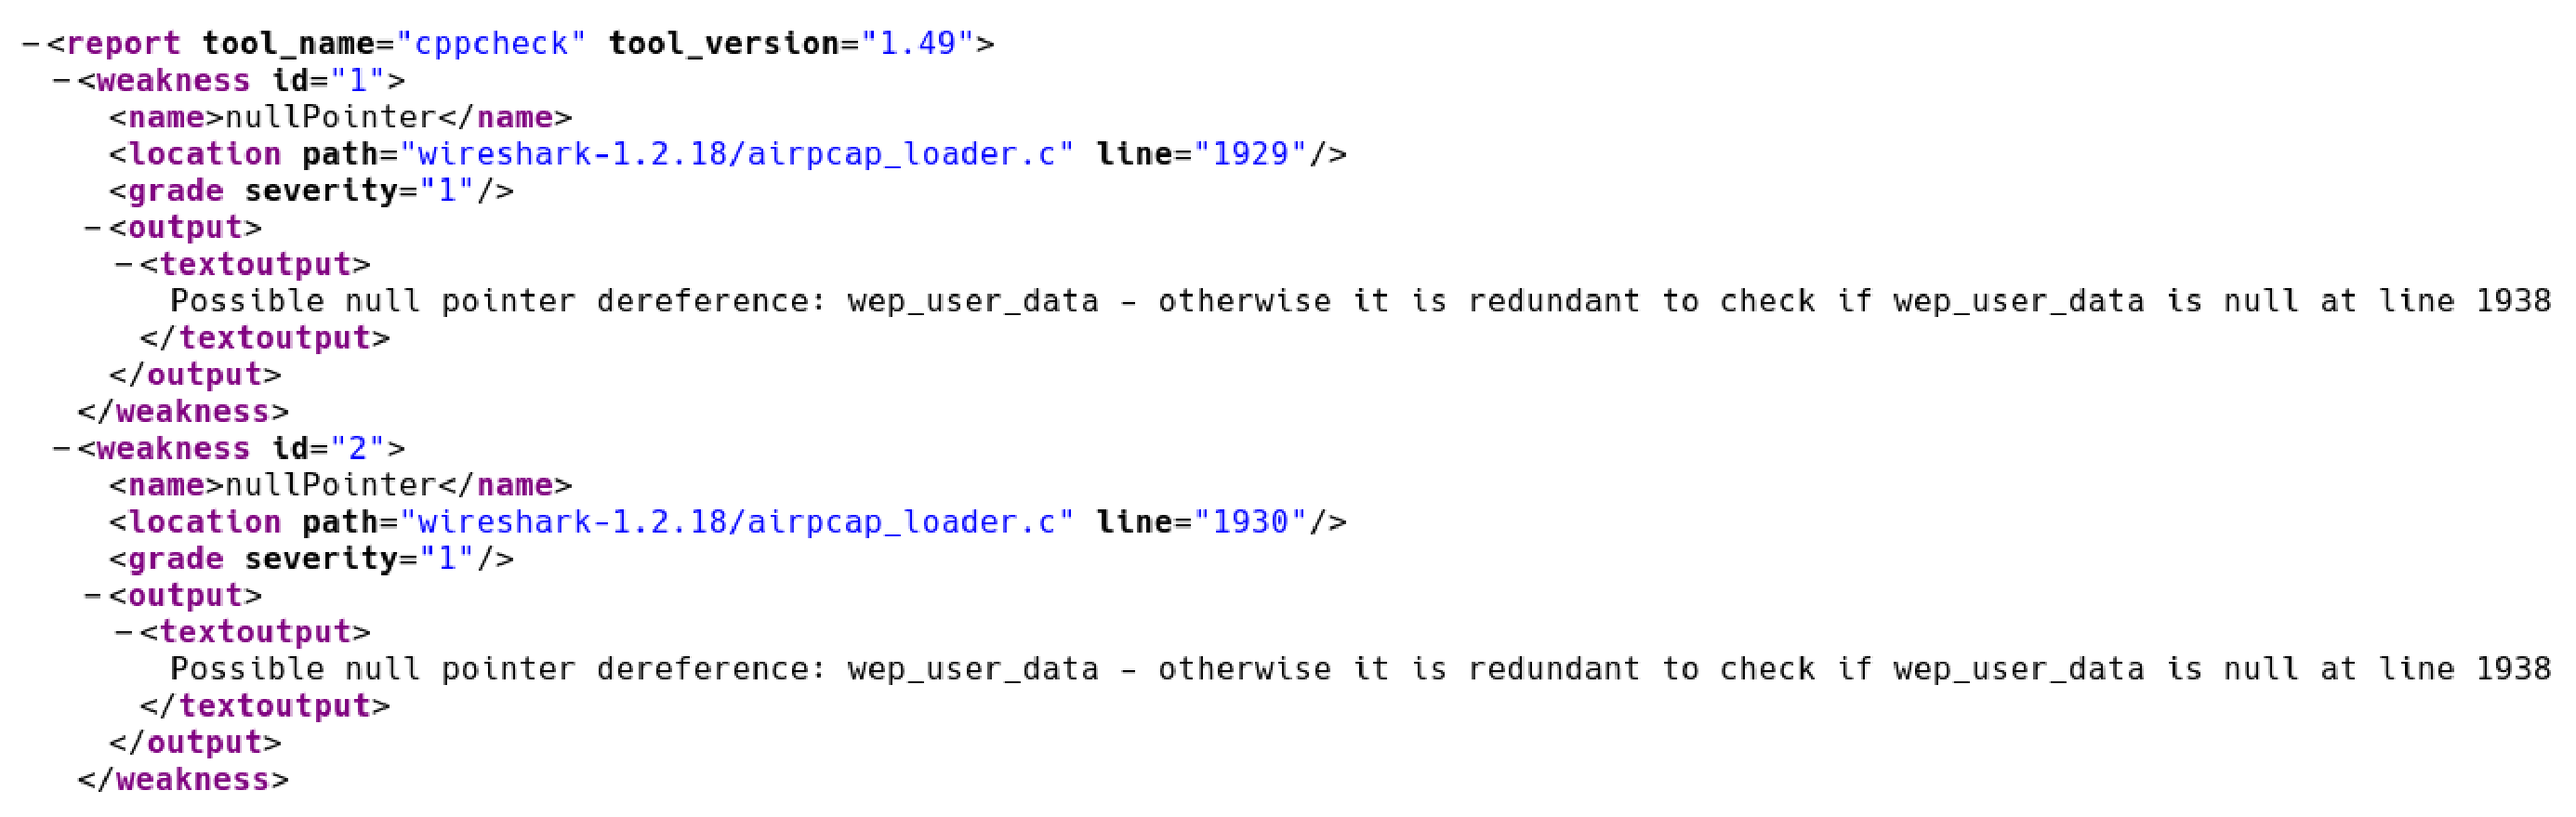
\includegraphics[scale=0.42]{figuras/cppcheck.eps}
	\caption{Exemplo de relatório da ferramenta cppcheck}
\end{figure}
\newpage

A primeira etapa do projeto foi a submissão dos relatórios gerados \ 
pelas ferramentas, utilizando o esquema da figura~\ref{sate_schema}. \ 
A segunda etapa foi a análise dos relatórios por parte de \ 
pesquisadores do $Mitre$ em conjunto com os envolvidos no projeto $Sate$. \ 
Uma das abordagens utilizadas nessa análise envolvia relacionar os \ 
problemas relatados pelas ferramentas a $CWE's$ catalogadas. \ 
Essa abordagem permitiu chegar as seguintes caracteríticas de uma $CWE$:

\begin{itemize}
        \item Pode ser associada com mais de uma $CWE$ ($CWE$ composta).
        \item Pode estar relacionada a mais de uma chamada no código fonte.
        \item Pode possuir mais de um fluxo de dados.
\end{itemize}

Os dados coletados por $Sate$, nos permite afirmar \ 
que: \emph{Estima-se que, apenas entre 1/8 e 1/3  de todas as \ 
fraquezas coletadas são simples.}

\subsection{Debile}

\subsection{Sloccount}


\section{Modelo probabilistico}
 Esta pesquisa tem por objetivo geral \
investigar de que maneira características intrinsicas de um projeto \
podem impactar na maneira como ferramentas de análise estática como o \ 
$Debile$ coletam fraquezas de software. Dessa maneira, podemos representar \
a visão geral deste problema de aprendizado da seguinte forma

\begin{figure}[h]
	\centering
	\label{visao_geral}
        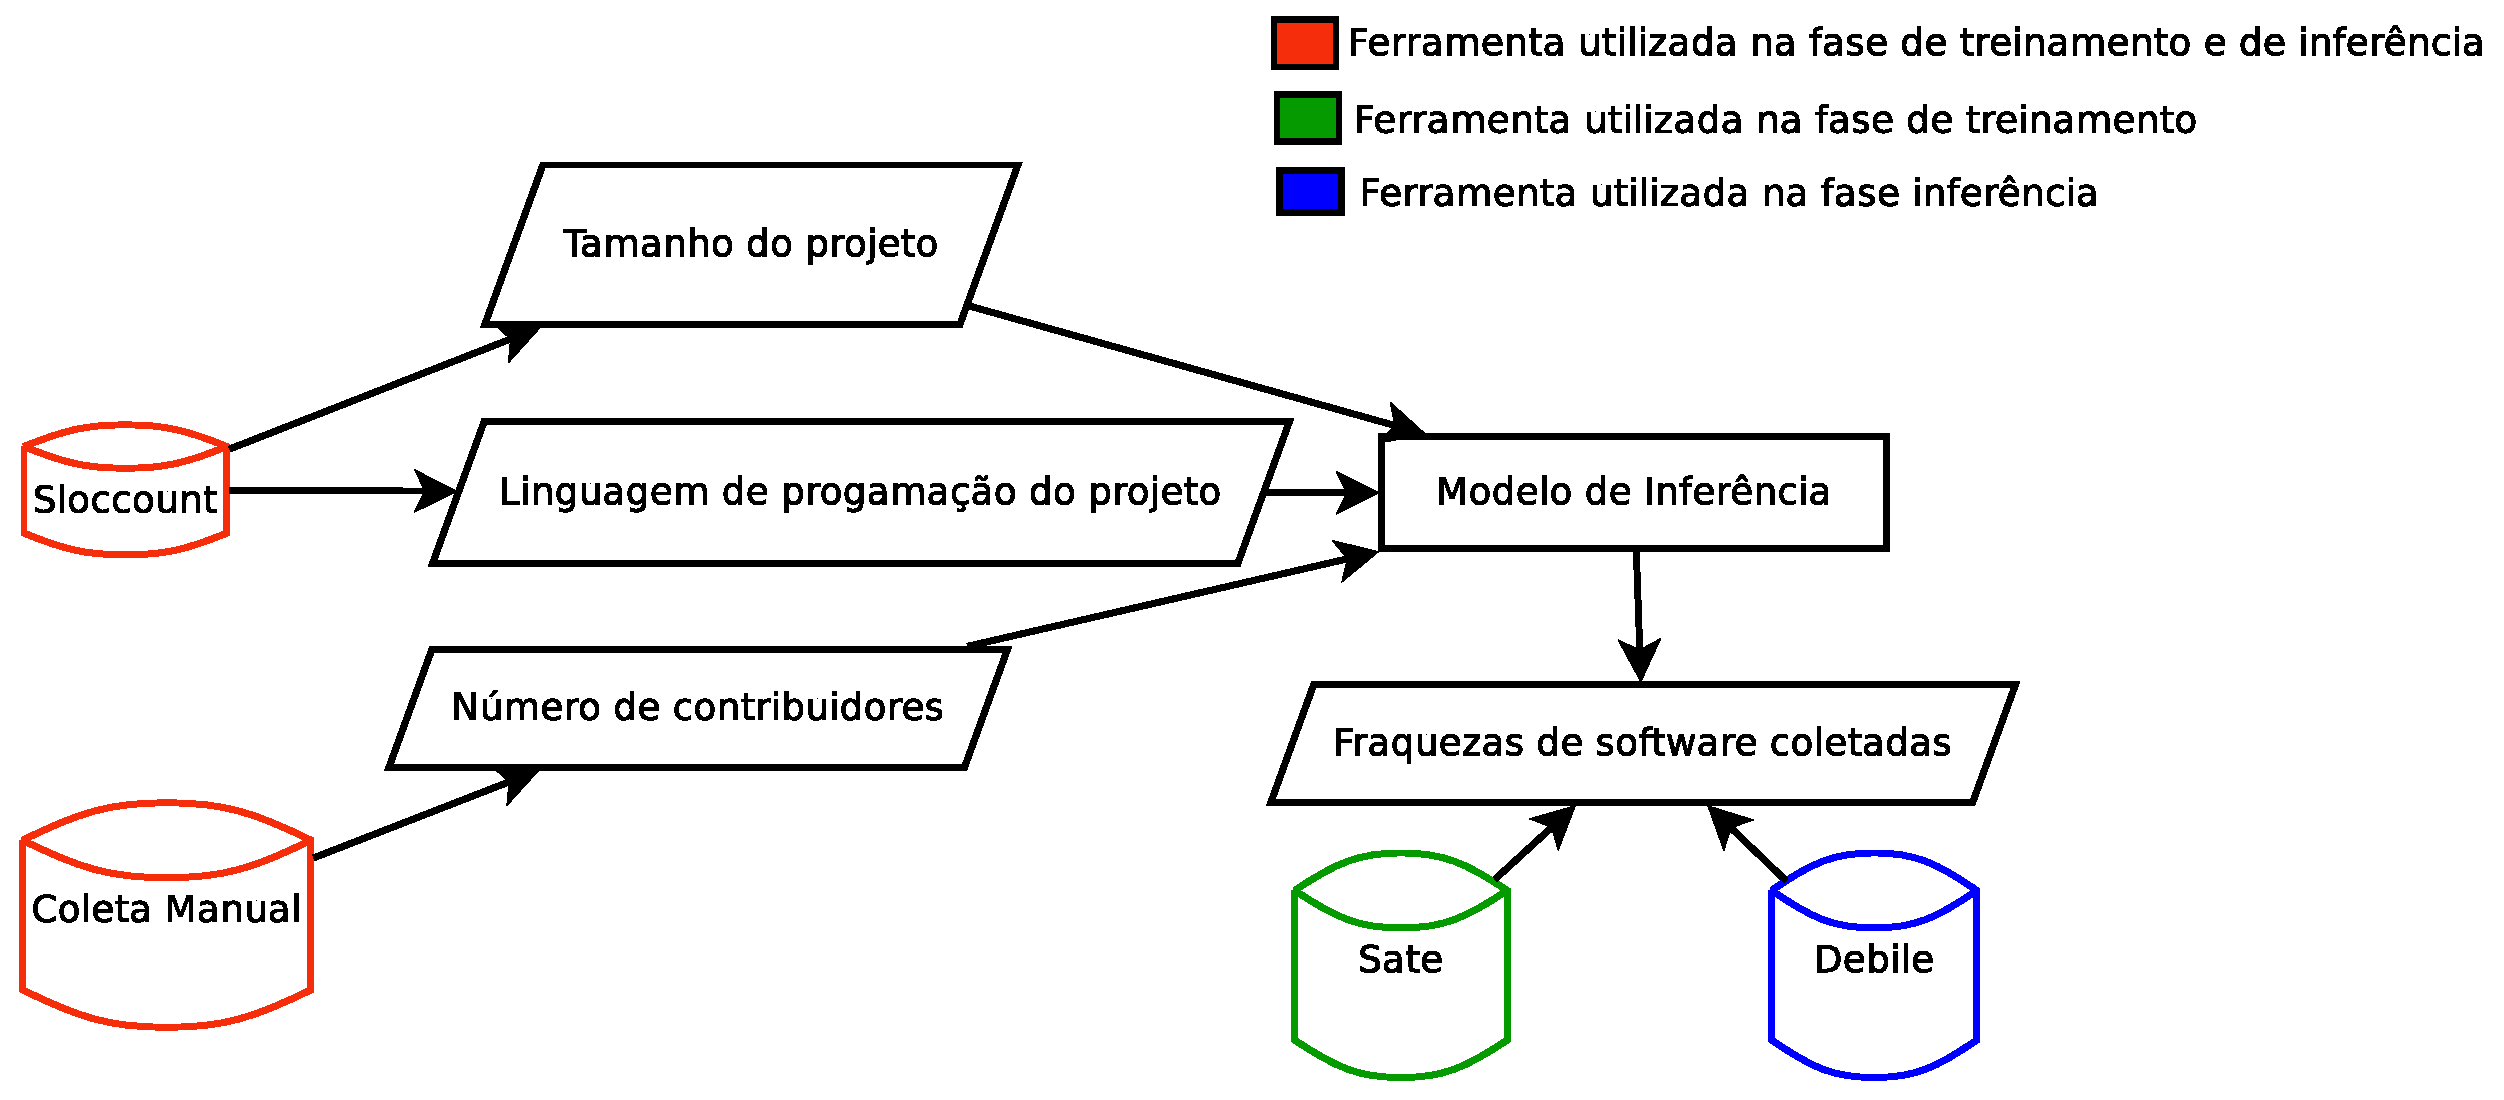
\includegraphics[scale=0.40]{figuras/visao_geral.eps}
	\caption{Abordagens para aprendizado de máquina}
\end{figure}

As fraquezas de software serão nossa variável $Y$, de maneira que iremos \
coletá-las utilizando as ferramentas $Sate$ e $Debile$. É preciso entender,
que um problema de aprendizado é dividido basicamente em duas etapas: treinamento e\ 
aplicação do modelo em dados novos, assim como é mostrado na \ 
figura~\ref{fluxo_treinamento}.  A figura ~\ref{visao_geral} demonstra \
quais serão as variáveis independentes do nosso modelo probabilistico: \
\[
X = \{tamanho\ do\ projeto, linguagem\ de\ programação, número\ de\ contribuidores\}
\]
$Y$ será o número de fraquezas encontradas pelas ferramentas que iremos \ 
utilizar tanto na fase de treinamento, quanto na fase de aplicação.  Para \ 
construirmos nosso modelo estatístico, utilizaremos a técnica \ 
de $regressão\ linear$, a partir do método de $mínimos\ quadrados$.

